\section{The problem}
Most reading devices for the blind, utilise sound output to convey the message to the reader.
However, this inhibits the individual's ability to hear their environment which is crucial when considering the reliance on sound and touch to get information about their surroundings.
Additionally, these devices are of no use for people suffering from deafblindness.

Although there are some devices in the market (figure \ref{fig:braille-readers-examples}) that allow the output of text in Braille form, they are expensive, ranging from GBP 1000 to GBP 5000, making them inacessible. Efforts have been made to produce more economical solutions and a variety of technologies have been utilised, however none of the many prototypes produced have reached the market.

This project aims to produce an affordable device to read and produce braille at home level.
By utilizing cheap electronics, such as off-the-shelf microcontrollers and push-pull solenoids, and using cheap manufacturing techniques to produce the casing and inner parts of the device, the cost can be kept reasonable for the customer.
Focus is placed on the device being suitable for both blind and deafblind individuals, and by using Braille instead of sound, there is an added privacy benefit to the user.
\begin{figure}[h]
\centering
    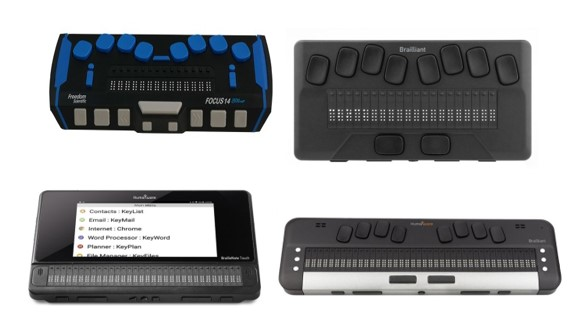
\includegraphics[width=0.7\textwidth]{figures/braille-readers-examples.jpg}
\caption{Different Braille generating devices. Prince range: GBP 1,637 (top left) to GBP 4,995 (bottom left)}
\label{fig:braille-readers-examples}
\end{figure}

\subsection{Stakeholders}
There are a variety of stakeholders that will benefit from such a device.
Firstly, people with visual impairment.
The design introduces a new and convenient way to read text allowing them to become more independent.
Particularly important for individuals with multisensory impairment, the solution must not rely on audio to convey the text to the reader.

As a result, family and friends of the visually impaired also benefit.
With their loved ones becoming more self-reliant, they are relieved from part of their duties that may have involved assisting with reading.
It provides them with a way to communicate in writing with their loved one without requiring the knowledge of braille.

The solution will provide small businesses the opportunity to become more inclusive without requiring big financial investments.
Ultimately, organisations such as the RNIB will be able to provide more tools that allow members to have a more normal and independent life.

It's worth mentioning we aim to compete with an existing industry of commercial braille embossing, who may try to inhibit the development and growth of such a braille printing/reading device.

\subsection{Objectives and criteria}
In order to keep costs low, cheap microcontrollers and manufacturing techniques are going to be utilised.
The device must be easily operatable by individuals who are visually and/or hearing impaired.
This can be achieved by, for example, using large buttons with embossed braille text that describe their function.

With a design focus of personal use, its size must be convenient to store or carry, and safe to use.
Additionally, the device's input and output must be easily identifiable and usable with minimal error.
This means that the device cannot have any sharp edges, and must effectively enclose wires and moving parts so as to hide such hazards from the user.
Finally, the device must not need special add-ons to operate.
This would go against the original idea of simplifying tasks for the visually impaired.
 

\subsection{Risks and constraints}
Manufacture and assembly of the prototype will be done in-house.
Injuries can cause delays to the manufacture, but can easily be avoided by following the established security protocols for the machines that will be utilised.
This includes, for example, appropriate utilisation of gloves, helmet and other protective equipment and using low currents for the circuit.
The device must also be built in a way that minimises the risk of injury when operated by a visually and possibly hearing-impaired person.

The limited availability and cost of appropriate parts may cause assembly setbacks and directly affect the mechanisms to be used.
For that reason, we are allowing some room for on-the-fly adjustment in the design of both software and hardware as necessary.
While we aim to include complicated capability, such as image-to-text conversion, we acknowledge the limited time and budget of the project, which may result in the development of only a proof of concept.

Training is expected to be provided to the user to ensure the correct usage and to allow for troubleshooting of simple operational issues (e.g. a printer having a paper jam).